\documentclass[a4paper]{article}
\usepackage[affil-it]{authblk}
\usepackage[backend=bibtex,style=numeric]{biblatex}
\usepackage{amsmath, amsthm, amssymb, amsfonts}
\usepackage{titlesec}
\usepackage{graphicx}
\usepackage{multirow}
\usepackage{hyperref}
\usepackage{cleveref}
\hypersetup{
    colorlinks=true,    % 彩色链接
    linkcolor=blue,      % 内部链接的颜色
    citecolor=red,      % 引用的颜色
    urlcolor=cyan       % 外部链接的颜色
}
\usepackage{geometry}
\usepackage[lined, ruled]{algorithm2e}
\geometry{margin=1.5cm, vmargin={0pt,1cm}}
\setlength{\topmargin}{-1cm}
\setlength{\paperheight}{29.7cm}
\setlength{\textheight}{25.3cm}
\titleformat{\section}{\Large\bfseries}{\Roman{section}}{1em}{}
\titleformat{\subsection}{\large\bfseries}{\Roman{section}.\alph{subsection}}{1em}{}
\titleformat{\subsubsection}{\normalsize\bfseries}{\Roman{section}.\alph{subsection}.\roman{subsubsection}}{1em}{}

\crefname{algorithm}{Algorithm}{Algorithms}
\Crefname{algorithm}{Algorithm}{Algorithms}
\crefname{equation}{Equation}{Equations}
\Crefname{equation}{Equation}{Equations}
\crefname{figure}{Figure}{Figures}
\Crefname{figure}{Figure}{Figures}
\crefname{table}{Table}{Tables}
\Crefname{table}{Table}{Tables}

\crefalias{algocf}{algorithm}

\renewcommand\arraystretch{1.2}

%\addbibresource{citation.bib}

\begin{document}
% =================================================
\title{\textbf{Numerical Analysis theoretical homework \# 3}}

\author{Peng Haowei 3220104816
  \thanks{E-mail address: \texttt{3220104816@zju.edu.cn}}}
\affil{(Information and Computing Science), Zhejiang University} 

\date{Due time: \today}

\maketitle

\section{Supplement the spline}

In this section, we consider $s \in \mathbb{S}_3^2$ on $[0, 2]$:
\begin{equation}
  s(x) = \begin{cases}
    p(x) ,& x \in [0, 1], \\
    (2 - x)^3 ,& x \in [1, 2].
  \end{cases}
  \label{eq:1_problem}
\end{equation}

\subsection{Determine $p$}

As $s(0) = 0$, we can assume that $p(x) = a_1 x + a_2 x^2 + a_3 x^3$ for $x \in [0, 1]$.

For $s \in \mathbb{S}_3^2$, we have
\begin{equation}
    p(1) = (2 - 1)^3 = 1,\
    p'(1) = -3*(2 - 1)^2 = -3,\
    p''(1) = 6*(2 - 1) = 6,
  \label{eq:1_p_derivatives}
\end{equation}
which yields
\begin{equation}
  \begin{cases}
    a_1 + a_2 + a_3 &= 1,\\
    a_1 + 2a_2 + 3a_3 &= -3, \\
    2a_2 + 6a_3 &= 6.
  \end{cases}
  \label{eq:1_p_coefficients}
\end{equation}

By solving the \cref{eq:1_p_coefficients}, we can get that 
\begin{equation}
  p(x) = 12x - 18x^2 + 7x^3.
  \label{eq:1_p_solution}
\end{equation}

\subsection{Judge the natural cubic spline}

According to the definition, a natural cubic spline $s \in \mathbb{S}_3^2$ satisfies boundary conditions
\begin{equation}
  s''(f; a) = 0,\ s''(f; b) = 0.
  \label{eq:1_natural_cubic_spline}
\end{equation}

Form \cref{eq:1_problem,eq:1_p_solution}, we can know that $s''(f; 0) = -36, s''(f; 2) = 0$, so $s(x)$ is not a natural cubic spline.

\section{Interpolate a function with a quadratic spline}

For this problem, we consider interpolating $f$ on $[a, b]$ with a quadratic spline $s \in \mathbb{S}_2^1$.

\subsection{The necessity of an additional condition}

With the Theorem 3.14, the set of splines $\mathbb{S}_2^1(x_1, x_2, \cdots, x_n)$ is a linear space with dimension $n + 1$. 
So only with the $f_1, f_2, \cdots, f_n$ and an additional condition, we get $n + 1$ conditions to determine the coefficients of the quadratic spline.

\subsection{Determine $p_i$ with the some conditions}

Denote $K_i = f[x_i, x_{i + 1}]$, so the table of divided difference for the Hermite interpolation problem $p_i(x_i) = f_i, p_i(x_{i + 1}) = f_{i + 1}, p'_i(x_i) = m_i$ is illustrated in \cref{tb:2_divided_difference}.

\begin{table}[htbp]
  \centering
  \begin{tabular}{c|ccc}
    $x_i$ & $f_i$ & & \\
    $x_i$ & $f_i$ & $m_i$ & \\
    $x_{i + 1}$ & $f_{i + 1}$ & $K_i$ & $\frac{K_i - m_i}{x_{i + 1} - x_i}$ \\
  \end{tabular}
  \caption{Divided difference table for the quadratic interpolation problem}
  \label{tb:2_divided_difference}
\end{table}

Then the Newton formula yields
\begin{equation}
  \begin{aligned}
    p_i(x) &= f_i + (x - x_i)m_i + (x - x_i)^2 \frac{K_i - m_i}{x_{i + 1} - x_i} \\
    &= f_i + (x - x_i)m_i + (x - x_i)^2 \frac{(f_{i + 1} - f_i)m_i}{(x_{i + 1} - x_i)^2}.
  \end{aligned}
  \label{eq:2_newton_formula}
\end{equation}

\subsection{Compute other derivatives with precondition $m_1$}

With \cref{eq:2_newton_formula} and $m_1 = f'(a)$, we can firstly get $p_1(x)$ and $p'_1(x)$.
As $s \in \mathbb{S}_2^1$, it follows that $p'_i(x_{i + 1}) = p'_{i + 1}(x_{i + 1})$, so with $p'_1$ we can get $m_2$. Similarly, we can get $m_3, m_4, \cdots, m_{n - 1}$.

\section{Determine a natural cubic spline}

In this task, we consider 
\begin{equation}
  s(x) = \begin{cases}
    s_1(x),& x \in [-1, 0], \\
    s_2(x),& x \in [0, 1], \\
  \end{cases}
\end{equation}
where $s_1(x) = 1 + c(x + 1)^3$ and $c \in \mathbb{R}$.

Assuming that $s_2(x) = a_0 + a_1 x + a_2 x^2 + a_3 x^3$, we can get $a_0 = 1 + c,\ a_1 = 3c,\ a_2 = 3c$ with $s_1(0) = 1 + c,\ s'_1(0) = 3c,\ s''_1(0) = 6c$. 
Then we get 
\begin{equation}
  \begin{aligned}
    s_2(x) &= a_3x^3 + 3cx^2 + 3cx + 1 + c, \\
    s''_2(x) &= 6a_3x + 6c.
  \end{aligned}
  \label{eq:3_s2_coefficients}
\end{equation}

According to the boundary conditions in \cref{eq:1_natural_cubic_spline}, we can get $s''_2(1) = 0$, which yields $a_3 + c = 0$. Then $s_2(x)$ follows
\begin{equation}
  s_2(x) = -cx^3 + 3cx^2 + 3cx + 1 + c,
  \label{eq:3_s2_solution}
\end{equation}
meaning that $s(1) = 6c + 1 = -1$. So the result is 
\begin{equation}
  c = -\frac{1}{3}.
  \label{eq:3_c_result}
\end{equation}

\section{Compare the spline with other interpolation polynomials}

The function we consider in this section is 
\begin{equation}
  \begin{aligned}
    f(x) &= \cos (\frac{\pi}{2}x), \\
    f'(x) &= -\frac{\pi}{2}\sin(\frac{\pi}{2}x),
  \end{aligned}
  \label{eq:4_problem}
\end{equation}
where $x \in [-1, 1]$.

\subsection{Interpolate $f$ with a natural cubic spline}

Denote the natural cubic spline interpolant to $f$ on knots $-1, 0, 1$ as 
\begin{equation}
  s(x) = \begin{cases}
    s_1(x),& x \in [-1, 0], \\
    s_2(x),& x \in [0, 1]. \\
  \end{cases}
  \label{eq:4_natural_cubic_spline}
\end{equation}

With the condition $s_1(0) = s_2(0) = 1,\ s'_1(0) = s'_2(0),\ s''_1(0) = s''_2(0)$, we can get the form of $s_1(x), s_2(x)$ with
\begin{equation}
  \begin{aligned}
    s_1(x) &= 1 + ax + bx^2 + c_1x^3, \\
    s_2(x) &= 1 + ax + bx^2 + c_2x^3. \\
  \end{aligned}
  \label{eq:4_natural_cubic_spline_coefficients}
\end{equation}

Besides, we have $s''_1(-1) = s''_1(1) = 0$ according to the boundary condition \cref{eq:1_natural_cubic_spline}, so the formula of $s(x)$ is 
\begin{equation}
  s(x) = \begin{cases}
    -\frac{1}{2} x^3 - \frac{3}{2} x^2 + 1,& x \in [-1, 0], \\
    \frac{1}{2} x^3 - \frac{3}{2} x^2 + 1,& x \in [0, 1]. \\
  \end{cases}
  \label{eq:4_natural_cubic_spline_solution}
\end{equation}

\subsection{Verify the minimal bending energy}

From \cref{eq:4_natural_cubic_spline_solution}, we can know that 
\begin{equation}
  [s''(x)]^2 = \begin{cases}
    9x^2 + 18x + 9,& x \in [-1, 0], \\
    9x^2 - 18x + 9,& x \in [0, 1]. \\
  \end{cases}
  \label{eq:4_minimal_bending_energy}
\end{equation}

So the bending energy of $s$ is 
\begin{equation}
  \int_{-1}^{1} [s''(x)]^2 \mathrm{d}x = 6
  \label{eq:4_bending_energy_s}
\end{equation}

\subsubsection{Compared with the quadratic polynomial}

The divided difference table for the quadratic interpolation problem is shown as follows.
\begin{table}[htbp]
  \centering
  \begin{tabular}{c|ccc}
    -1 & 0 &    &    \\
    0  & 1 & 1  &    \\
    1  & 0 & -1 & -1 \\
  \end{tabular}
  \caption{Divided difference table for the quadratic interpolation problem}
  \label{tb:4_divided_difference_quadratic}
\end{table}
So the quadratic interpolation polynomial is
\begin{equation}
  p(x) = 1 \cdot (x + 1) - x(x + 1) = 1 - x^2,
  \label{eq:4_quadratic_polynomial}
\end{equation}
and its bending energy is 
\begin{equation}
  \int_{-1}^{1} [p''(x)]^2 \mathrm{d}x = \int_{-1}^1 (1 - 2x^2 + x^4) \mathrm{d}x = 8 > 6,
\end{equation}
which verifies $s$ holds the smaller energy.

\subsubsection{Compared with the initial function $f$}

The bending energy of $f$ is 
\begin{equation}
  \int_{-1}^{1} [f''(x)]^2 \mathrm{d}x = \int_{-1}^1 \frac{\pi^4}{16}\cos^2 (\frac{\pi}{2}x) = \frac{\pi^4}{16} \approx 6.09 > 6,
\end{equation}
which means that $s$ holds the smaller energy as well.

\section{Problems about the quadratic B-spline $B_i^2(x)$}

\subsection{Derive the explicit expression of $B_i^2(x)$}

According to the Definition 3.23 in our textbook, B-spline $B_i^2(x)$ is defined recursively by
\begin{equation}
  B_i^2(x) = \frac{x - t_{i - 1}}{t_{i + 1} - t_{i - 1}}B_i^n(x) + \frac{t_{i + 2} - x}{t_{i + 2} - t_i}B_{i + 1}^1(x).
  \label{eq:5_B_spline_definition}
\end{equation}

Meanwhile, the Definition 3.21 gives us the definition of the hat function, so it follows
\begin{equation}
  \hat{B}_i(x) = \begin{cases}
    \frac{x - t_{i - 1}}{t_i - t_{i - 1}},& x \in (t_{i - 1}, t_i], \\
    \frac{t_{i + 1} - x}{t_{i + 1} - t_{i}},& x \in (t_i, t_{i + 1}], \\
    0,& \text{otherwise}, \\
  \end{cases}
  \label{eq:5_hat_B_spline_definition}
\end{equation}
and we have $B_i^1 = \hat{B}_i$.

With the above equations, we can get the explicit expression of $B_i^2(x)$ as
\begin{equation}
  \begin{aligned}
    B_i^2(x) &= \frac{x - t_{i - 1}}{t_{i + 1} - t_{i - 1}}B_i^n(x) + \frac{t_{i + 2} - x}{t_{i + 2} - t_i}B_{i + 1}^1(x) \\
    &= \frac{x - t_{i - 1}}{t_{i + 1} - t_{i - 1}} \hat{B}_i(x) + \frac{t_{i + 2} - x}{t_{i + 2} - t_i} \hat{B}_{i + 1}(x) \\
    &= \begin{cases}
      \frac{(x - t_{i - 1})^2}{(t_{i + 1} - t_{i - 1})(t_i - t_{i - 1})},& x \in (t_{i - 1}, t_i]; \\
      \frac{(x - t_{i - 1})(t_{i + 1} - x)}{(t_{i + 1} - t_{i - 1})(t_{i + 1} - t_i)} + \frac{(t_{i + 2} - x)(x - t_i)}{(t_{i + 2} - t_i)(t_{i + 1} - t_i)},& x \in (t_i, t_{i + 1}]; \\
      \frac{(t_{i + 2} - x)^2}{(t_{i + 2} - t_i)(t_{i + 2} - t_{i + 1})},& x \in (t_{i + 1}, t_{i + 2}]; \\
      0,& \text{otherwise}. \\
    \end{cases}
  \end{aligned}
  \label{eq:5_B_spline_explicit_expression}
\end{equation}

\subsection{Verify the continuity at knots}

As the $B_i^2(x)$ is polynomial, we can verify its piecewise-differentiability. The derivative of $B_i^2(x)$ follows
\begin{equation}
  \frac{\mathrm{d}B_i^2(x)}{\mathrm{d}x} = \begin{cases}
    \frac{2(x - t_{i - 1})}{(t_{i + 1} - t_{i - 1})(t_i - t_{i - 1})},& x \in (t_{i - 1}, t_i]; \\
    \frac{-2x + t_{i - 1} + t_{i + 1}}{(t_{i + 1} - t_{i - 1})(t_{i + 1} - t_i)} + \frac{-2x + t_i + t_{i + 2}}{(t_{i + 2} - t_i)(t_{i + 1} - t_i)},& x \in (t_i, t_{i + 1}]; \\
    \frac{-2(t_{i + 2} - x)}{(t_{i + 2} - t_i)(t_{i + 2} - t_{i + 1})},& x \in (t_{i + 1}, t_{i + 2}]; \\
    1,& \text{otherwise}. \\
  \end{cases}
  \label{eq:5_B_spline_derivative}
\end{equation}

With the \cref{eq:5_B_spline_derivative}, the left-hand and right-hand derivative of $t_i$ and $t_{i + 1}$ are
\begin{equation}
  \begin{aligned}
    \frac{\mathrm{d}B_i^2}{\mathrm{d}x}(t_i) &= \frac{2}{t_{i + 1} - t_{i - 1}}, \\ 
    \frac{\mathrm{d}B_i^2}{\mathrm{d}x}(t_i+) &= \frac{-2t_i + t_{i - 1} + t_{i + 1}}{(t_{i + 1} - t_{i - 1})(t_{i + 1} - t_i)} - \frac{1}{(t_{i + 1} - t_i)} = \frac{2}{t_{i + 1} - t_{i - 1}}, \\ 
    \frac{\mathrm{d}B_i^2}{\mathrm{d}x}(t_{i + 1}) &= -\frac{1}{(t_{i + 1} - t_i)} + \frac{-2t_{i + 1} + t_i + t_{i + 2}}{(t_{i + 2} - t_i)(t_{i + 1} - t_i)} = \frac{-2}{t_{i + 2} - t_i}, \\
    \frac{\mathrm{d}B_i^2}{\mathrm{d}x}(t_{i + 1}+) &= \frac{-2}{t_{i + 2} - t_i}, \\
  \end{aligned}
  \label{eq:5_B_spline_derivative_at_knots}
\end{equation}
which implies the continuity of $B_i^2(x)$ at $t_i$ and $t_{i + 1}$.

\subsubsection{Show the unique zero of the derivative and express it}

Obviously, the derivative of $B_i^2(x)$ has no zero on the interval $(t_{i - 1}, t_i)$. On the interval $[t_i, t_{i + 1})$, the derivative is a linear function and it changes signature because of 
\begin{equation}
  \frac{\mathrm{d}B_i^2}{\mathrm{d}x}(t_i) \cdot \frac{\mathrm{d}B_i^2}{\mathrm{d}x}(t_{i + 1}) = \frac{2}{t_{i + 1} - t_{i - 1}} \cdot \frac{-2}{t_{i + 2} - t_i} < 0,
  \label{eq:5_B_spline_derivative_sign}
\end{equation}
so the derivative has a unique zero $x^*$ on $(t_{i - 1}, t_{i + 1})$.

Solving $\frac{-2x + t_{i - 1} + t_{i + 1}}{(t_{i + 1} - t_{i - 1})(t_{i + 1} - t_i)} + \frac{-2x + t_i + t_{i + 2}}{(t_{i + 2} - t_i)(t_{i + 1} - t_i)} = 0$, we get the zero
\begin{equation}
  x^* = \frac{t_{i + 2}t_{i + 1} - t_it_{i - 1}}{t_{i + 2} + t_{i + 1} - t_i - t_{i - 1}}.
  \label{eq:5_B_spline_zero_of_derivative}
\end{equation}

\subsection{Show the range of $B_i^2(x)$}

We can easily get that $B_i^2(x) \geqslant 0$, so we only need to proof the spline is smaller than 1.

For the interval $(t_{i - 1}, t_i]$ and $(t_{i + 1}, t_{i + 2}]$, it is obvious that $B_i^2(x) < 1$. For the interval $[t_i, t_{i + 1})$, the maximum value occurs in $x = x^*$.
Assuming $B_i^2(x^*) \leqslant 1$, we have
\begin{equation}
  (x^* - t_{i - 1})(t_{i + 1} - x^*)(t_{i + 2} - t_i) + (t_{i + 2} - x^*)(x^* - t_i)(t_{i + 1} - t_{i - 1}) \geqslant (t_{i + 1} - t_{i - 1})(t_{i + 1} - t_i)(t_{i + 2} - t_i).
  \label{eq:5_B_spline_range_proof}
\end{equation}

According to Cauchy inequality, we have
\begin{equation}
  \begin{aligned}
    (x^* - t_{i - 1})(t_{i + 1} - x^*) \leqslant \frac{1}{4}(t_{i + 1} - t_{i - 1})^2, \\
    (t_{i + 2} - x^*)(x^* - t_i) \leqslant \frac{1}{4}(t_{i + 2} - t_i)^2. \\
  \end{aligned}
  \label{eq:5_B_spline_range_proof_2}
\end{equation}
So the left hand of \cref{eq:5_B_spline_range_proof} is less than $(t_{i + 1} - t_{i - 1})(t_{i + 2} - t_i)(t_{i + 2} + t_{i + 1} - t_i - t_{i - 1})$. Therefore, 
\begin{equation}
  \begin{aligned}
    (x^* - t_{i - 1})(t_{i + 1} - x^*)(t_{i + 2} - t_i) + (t_{i + 2} - x^*)(x^* - t_i)(t_{i + 1} - t_{i - 1}) &< \frac{1}{4}(t_{i + 1} - t_{i - 1})(t_{i + 2} - t_i)(t_{i + 2} + t_{i + 1} - t_i - t_{i - 1}) 
    &< (t_{i + 1} - t_{i - 1})(t_{i + 1} - t_i)(t_{i + 2} - t_i),
  \end{aligned}
  \label{eq:5_B_spline_range_proof_3}
\end{equation}
which leads to contradiction. Consequently, $B_i^2(x) \in [0, 1)$.

\subsection{Plot a figure of $B_i^2(x)$}

The figure of $B_i^2(x)$ for $t_i = i$ is shown as follows.

\begin{figure}[htbp]
  \centering
  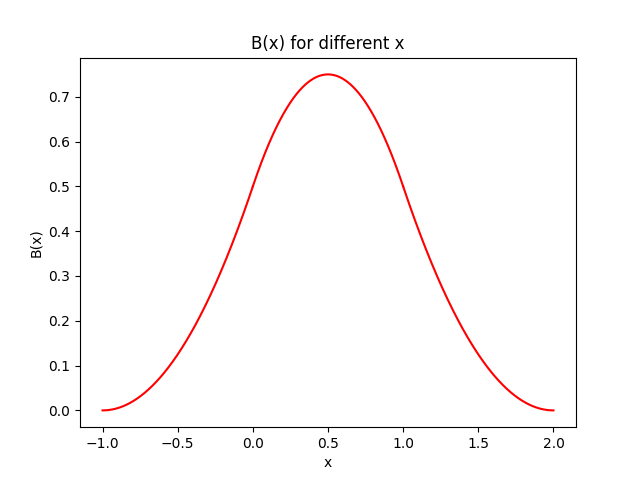
\includegraphics[width = 0.5\textwidth]{../images/B(x).png}
  \caption{The figure of $B_i^2(x)$ for $t_i = i$.}
  \label{fig:5_B_spline_figure}
\end{figure}

\section{Proof for Theorem 3.32 for $n = 2$}

\begin{proof}
  The exact formula of $B_i^2(x)$ is shown in \cref{eq:5_B_spline_explicit_expression}. For the target equation, 
  \begin{equation}
    \begin{aligned}
      & (t_{i + 2} - t_{i - 1})[t_{i - 1}, t_{i}, t_{i + 1}, t_{i + 2}](t - x)_{+}^2 \\
      =& [t_i, t_{i + 1}, t_{i + 2}](t - x)_{+} - [t_{i - 1}, t_{i}, t_{i + 1}](t - x)_{+} \\
      =& [t_{i + 1}, t_{i + 2}](t - x)_{+} - [t_{i}, t_{i + 1}](t - x)_{+} - [t_i, t_{i + 1}](t - x)_{+} + [t_{i - 1}, t_i](t - x)_{+} \\
      =& \frac{(t_{i + 2} - x)_{+} - (t_{i + 1} - x)_{+}}{t_{i + 2} - t_{i + 1}} - 2\frac{(t_{i + 1} - x)_{+} - (t_{i} - x)_{+}}{t_{i + 1} - t_{i}} + \frac{(t_i - x)_{+} - (t_{i - 1} - x)_{+}}{t_i - t_{i - 1}} \\
      =& \begin{cases}
        \frac{(x - t_{i - 1})^2}{(t_{i + 1} - t_{i - 1})(t_i - t_{i - 1})},& x \in (t_{i - 1}, t_i]; \\
        \frac{(x - t_{i - 1})(t_{i + 1} - x)}{(t_{i + 1} - t_{i - 1})(t_{i + 1} - t_i)} + \frac{(t_{i + 2} - x)(x - t_i)}{(t_{i + 2} - t_i)(t_{i + 1} - t_i)},& x \in (t_i, t_{i + 1}]; \\
        \frac{(t_{i + 2} - x)^2}{(t_{i + 2} - t_i)(t_{i + 2} - t_{i + 1})},& x \in (t_{i + 1}, t_{i + 2}]; \\
        0,& \text{otherwise}. \\        
      \end{cases} \\
      =& B_i^2(x).
    \end{aligned}
    \label{eq:6_proof}
  \end{equation}
\end{proof}

\section{Proof for the independence of the scaled integral}

In this section, we need to prove the scaled integral of a B-spline $B_i^n(x)$ over its support is independent of its index $i$ even if the spacing of the knots is not uniform, i.e.
\begin{equation}
  \frac{1}{t_{i + n} - t_{i - 1}} \int_{t_{i - 1}}^{t_{i + n}} B_i^n(x) \mathrm{d}x = \frac{1}{n + 1}.
  \label{eq:7_target_equation}
\end{equation}

\begin{proof}
  We prove the target equation by induction on $n$. For $n = 0$, the scaled integral is 
  \begin{equation}
    \frac{1}{t_i - t_{i - 1}} \int_{t_{i - 1}}^{t_n} B_i^0(x) \mathrm{d}x = \frac{1}{t_i - t_{i - 1}} \cdot (t_i - t_{i - 1}) = 1 = \frac{1}{n + 1}.
    \label{eq:7_scaled_integral_n_0}
  \end{equation}

  Then we assume that the \cref{eq:7_target_equation} holds for $n \leqslant k$. For $n = k + 1$, the scaled integral is
  \begin{equation}
    \begin{aligned}
      & \int_{t_{i - 1}}^{t_{i + k + 1}} B_i^{k + 1}(x) \mathrm{d}x \\
      =& x B_i^{k + 1}(x) \big|_{t_{i - 1}}^{t_{i + k + 1}} - \int_{t_{i - 1}}^{t_{i + k}} x \frac{\mathrm{d}}{\mathrm{d}x} B_i^{k + 1}(x) \mathrm{d}x \\
      =& - \int_{t_{i - 1}}^{t_{i + k + 1}} x \left(\frac{(k + 1)B_i^k(x)}{t_{i + k} - t_{i - 1}} - \frac{(k + 1)B_{i + 1}^k(x)}{t_{i + k + 1} - t_i}\right) \mathrm{d}x \\
      =& -(k + 1) \int_{t_{i - 1}}^{t_{i + k + 1}} B_i^{k + 1}(x) + \frac{t_{i - 1}}{t_{i + k} - t_{i - 1}}B_i^k(x) - \frac{t_{i + k + 1}}{t_{i + k + 1} - t_i} B_{i + 1}^k(x) \mathrm{d}x. \\
    \end{aligned}
    \label{eq:7_scaled_integral_n_k+1}
  \end{equation}
  Then we get
  \begin{equation}
    \begin{aligned}
      & \int_{t_{i - 1}}^{t_{i + k + 1}} B_i^{k + 1}(x) \mathrm{d}x \\
      =& \frac{1}{k + 2} \int_{t_{i - 1}}^{t_{i + k + 1}} -\frac{t_{i - 1}}{t_{i + k} - t_{i - 1}}B_i^k(x) + \frac{t_{i + k + 1}}{t_{i + k + 1} - t_i} B_{i + 1}^k(x) \mathrm{d}x \\
      =& \frac{1}{k + 2} \int_{t_i}^{t_{i + k + 1}} \frac{t_{i + k + 1}}{t_{i + k + 1} - t_i} B_{i + 1}^k(x) \mathrm{d}x - \frac{1}{k + 2} \int_{t_{i - 1}}^{t_{i + k}} \frac{t_{i - 1}}{t_{i + k} - t_{i - 1}}B_i^k(x) \mathrm{d}x \\
      =& \frac{1}{k + 2} (t_{i + k + 1} - t_i). \\
    \end{aligned}
    \label{eq:7_scaled_integral_n_k+1_2}
  \end{equation}
  Therefore, the \cref{eq:7_target_equation} holds for $n = k + 1$, so the equation holds for all $n$.
\end{proof}

\section{Prove the theorem connecting complete symmetric polynomials and divided difference of monomials}

The theorem waiting for proving is
\begin{align}
  \forall m \in \mathbb{N}^+,\ \forall i \in \mathbb{N},\ & \forall n = 0, 1, \cdots, m, \notag \\ 
  \tau_{m - n} (x_i, \cdots, x_{i + n}) &= [x_i, \cdots, x_{i + n}]x^m. \label{eq:8_theorem}
\end{align}

\subsection{Verify the theorem for $m = 4,\ n = 2$}

The table of divided difference is illustrated as follows.
\begin{table}[htbp]
  \centering
  \begin{tabular}{c|cccc}
    $x_1$ & $x_1^4$ &        &        &        \\ 
    $x_2$ & $x_2^4$ & $x_1^3 + x_1^2 x_2 + x_1 x_2^2 + x_2^3$ &        &        \\ 
    $x_3$ & $x_3^4$ & $x_2^3 + x_2^2 x_3 + x_2 x_3^2 + x_3^3$ & $x_1^2 + x_1x_3 + x_3^2 + x_2(x_1 + x_3) + x_2^2$ &        \\ 
    $x_4$ & $x_4^4$ & $x_3^3 + x_3^2 x_4 + x_3 x_4^2 + x_4^3$ & $x_2^2 + x_2x_4 + x_4^2 + x_3(x_2 + x_4) + x_3^2$ & $x_1 + x_2 + x_3 + x_4$ \\ 
  \end{tabular}
  \caption{Divided difference of $x^4$ with $x_1, x_2, x_3, x_4$ as the four knots.}
  \label{tab:8_divided_difference}
\end{table}

From \cref{tab:8_divided_difference}, we get $[x_1, x_2, x_3]x^4 = x_1^2 + x_1x_3 + x_3^2 + x_2(x_1 + x_3) + x_2^2 = x_1x_2 + x_1x_3 + x_2x_3 + x_1^2 + x_2^2 + x_3^2 = \tau(x_1, x_2, x_3)$. 
Other condition cna be proved similarly.

So \cref{eq:8_theorem} is verified for $m = 4,\ n = 2$.

\subsection{Prove the theorem by Lemma 3.45}

The lemma mentioned is 
\begin{equation}
  \tau_{k + 1}(x_1, \cdots, x_n, x_{n + 1}) = \tau_{k + 1}(x_1, \cdots, x_n) + x_{n + 1}\tau_k(x_1, \cdots, x_n, x_{n + 1}).
  \label{eq:8_lemma}
\end{equation}

\begin{proof}

  Before the proof by induction, we firstly have
  \begin{equation}
    \begin{aligned}
      & (x_{n + i} - x_i)\tau_{k}(x_1, \cdots, x_n, x_{n + i}) \\
      =& \tau_{k + 1}(x_i, \cdots, x_n, x_{n + i}) - \tau_{k + 1}(x_i, \cdots, x_{i + n}) - x_i\tau_{k}(x_i, \cdots, x_{i + n}, x_{i + n + 1}) \\
      =& \tau_{k + 1}(x_{i + 1}, \cdots, x_n, x_{n + i}) + x_i \tau_k(x_i, \cdots, x_{i + n}, x_{i + n + 1}) - \tau_{k + 1}(x_i, \cdots, x_{i + n}) - x_i\tau_{k}(x_i, \cdots, x_{i + n}, x_{i + n + 1}) \\
      =& \tau_{k + 1}(x_{i + 1}, \cdots, x_n, x_{n + i}) - \tau_{k + 1}(x_i, \cdots, x_{i + n})
    \end{aligned}
    \label{eq:8_lemma_1}
  \end{equation}

  We prove this theorem by induction on $n$. For $n = 0$, we have
  \begin{equation}
    \tau_m(x_i) = x_i^m = [x_i]x^m.
    \label{eq:8_induction_base}
  \end{equation}
  
  Then we assume that the \cref{eq:8_theorem} holds for $n \leqslant k \ (k < m)$. For $n = k + 1$, we have
  \begin{equation}
    \begin{aligned}
      & \tau_{m - k - 1}(x_i, \cdots, x_{i + k}, x_{i + k + 1})   \\
      =& \frac{\tau_{m - k}(x_{i + 1}, \cdots, x_{i + k + 1}) - \tau_{m - k}(x_i, \cdots, x_{i + k})}{x_{i + k + 1} - x_i} \\
      =& \frac{[x_{i + 1}, \cdots, x_{i + k + 1}]x^m - [x_i, \cdots, x_{i + k}]x^m}{x_{i + k + 1} - x_i} \\
      =& [x_i, \cdots, x_{i + k + 1}]x^m,
    \end{aligned}
    \label{eq:8_lemma_2}
  \end{equation}
  which completes the proof by the induction.
\end{proof}

\section*{ \center{\normalsize {Acknowledgement}} }

In the process of writing this report, I use \href{https://kimi.moonshot.cn/}{\textit{Kimi AI}} to help me translate something and write this report by \TeX.

%\printbibliography

\end{document}
